% !TeX spellcheck = en_GB
\documentclass[a4paper]{tufte-handout}
\usepackage{amsmath,amsthm,amssymb}
\usepackage[tt=false]{libertine}
\usepackage{libertinust1math}
\usepackage[T1]{fontenc}
\usepackage{enumitem}
\usepackage{graphicx} % Required for inserting images
\usepackage{ifthen}
\usepackage{listings}
\usepackage{siunitx-v2}
\usepackage{subcaption}
\usepackage[most]{tcolorbox}
\usepackage{xcolor}
\usepackage{tikz}

%\usepackage[colorlinks, linkcolor=black]{hyperref}

%\addbibresource{references.bib}

%\numberwithin{equation}{section}

\DeclareCaptionFormat{custom}
{%
	{\sf\footnotesize\textbf{#1#2}{#3}}
}
\captionsetup{format=custom}

% Margin paragraphs
%\let\oldmarginpar\marginpar
%\setlength\marginparwidth{3cm}
%\renewcommand{\marginpar}[1]{\oldmarginpar{\flushleft\tiny\sf{#1}}}

% Colors
\definecolor{primary}{HTML}{5080da}
\definecolor{secondary}{HTML}{da8050}

% tikz definitions
\tikzset{leaf node/.style = {rectangle, draw=black, minimum width = 0.5cm, minimum height = 0.5cm}}
\tikzset{internal node/.style = {circle, draw=black, minimum width = 0.5cm}}

% Theorems
\newtcbtheorem{definition}{Definition}{colback=primary!5, colframe=primary, fonttitle=\bfseries}{def}
\newtcbtheorem{alert}{Alert}{colback=secondary!5, colframe=secondary, fonttitle=\bfseries}{alert}

\theoremstyle{definition}
\newtheorem{exercise}{Exercise}

% Code listings

\definecolor{codegreen}{rgb}{0,0.6,0}
\definecolor{codegray}{rgb}{0.5,0.5,0.5}
\definecolor{codepurple}{rgb}{0.58,0,0.82}
\definecolor{backcolour}{rgb}{0.95,0.95,0.92}

\lstdefinestyle{mystyle}{
	backgroundcolor=\color{backcolour},   
	commentstyle=\color{codegreen},
	keywordstyle=\color{magenta},
	numberstyle=\tiny\color{codegray},
	stringstyle=\color{codepurple},
	basicstyle=\ttfamily\footnotesize,
	breakatwhitespace=false,         
	breaklines=true,                 
	captionpos=b,                    
	keepspaces=true,                 
	numbers=left,                    
	numbersep=5pt,                  
	showspaces=false,                
	showstringspaces=false,
	showtabs=false,                  
	tabsize=2
}

\lstset{style=mystyle}

% Custom commands
\newcommand{\Z}{\mathbb{Z}}
\newcommand{\hint}{\textit{Hint:}~}
\newcommand{\inlcd}[1]{\lstinline[language=Python]{#1}}

% inline code blocks
\newcommand\mystrut{\rule[-1pt]{0pt}{.8em}}

\newtcbox{\code}{on line, boxrule=0pt, boxsep=0pt, top=2pt,
	left=2pt, bottom=2pt, right=2pt, colback=gray!25, colframe=white,
	fontupper={\ttfamily\mystrut}}

% Tikz settings
\usetikzlibrary{calc}
\usetikzlibrary{positioning}
\usetikzlibrary{matrix}

\tikzset{
	list/.style={
		matrix of math nodes,
		nodes in empty cells,
	},
}

\title{Functional Programming\\{\normalsize Revision Lab 01}}
\author{V. Markos\\{\normalsize Mediterranean College}}
\date{}

\begin{document}
	%
	\maketitle
	%
	\begin{abstract}
		First Functional Programming revision lab, with a focus on recursion, sorting, and\ldots pancakes. The main aim of this lab is to help reorganise any concepts explored so far.
	\end{abstract}
	%
	%
	%
	\section{Warm Up}
	%
	A few exercises to get us started, with a focus on recursion and simple list operations. As a set of guidelines for this and all upcoming exercises, do use function signatures and, where needed, utilise list comprehensions appropriately.
	
	\begin{exercise}
		Write a function named \code{max'} that returns the maximum element of a list. Then implement a tail recursive version, \code{max'{'}}.
	\end{exercise}

	\begin{exercise}
		Write a function named \code{sum'} that computes the sum of the elements of a list of floats. Then implement a tail recursive version, \code{sum'{'}}.
	\end{exercise}

	\begin{exercise}
		Write a function named \code{fib} that computes the $n$--th term of the Fibonacci sequence. As a reminder the $n$--th term of the Fibonacci sequence is given by:
		\begin{equation}
			f_{n}=f_{n-1}+f_{n-2},
		\end{equation}
		with $f_0=0$ and $f_1=1$. The first ten terms, thus, read:
		\[0,1,1,2,3,5,8,13,21,34.\]
	\end{exercise}

	As you might have observed, running the function \code{fib} for large inputs is quite slow. Can you explain why?
	
	\begin{exercise}
		As \code{fib} is too slow, given duplicated recursive function calls, we should devise a more optimal solution. To do so, implement a \emph{tail recursive} solution, where you use auxiliary arguments appropriately to keep track of the current Fibonacci value and anything else you might find useful. You can use \code{:set +s} in GHCi to print timing and memory data. What do you observe? 
	\end{exercise}

	\section{Merge Sort}
	%	
	\begin{marginfigure}
		\centering
		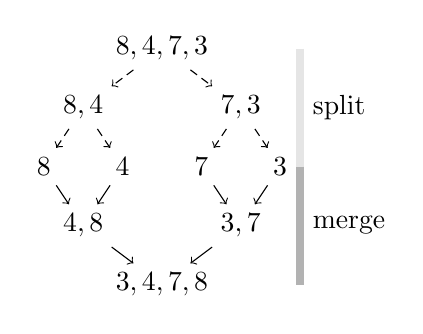
\begin{tikzpicture}[xscale=0.5, yscale=0.5]
			\node[rectangle] (0) at (0,0) {$8,4,7,3$};
			\node[rectangle] (00) at (-2,-1.5) {$8,4$};
			\node[rectangle] (01) at (2,-1.5) {$7,3$};
			\node[rectangle] (000) at (-3,-3) {$8$};
			\node[rectangle] (001) at (-1,-3) {$4$};	
			\node[rectangle] (010) at (1,-3) {$7$};
			\node[rectangle] (011) at (3,-3) {$3$};
			\node[rectangle] (10) at (-2,-4.5) {$4,8$};
			\node[rectangle] (11) at (2,-4.5) {$3,7$};
			\node[rectangle] (1) at (0,-6) {$3,4,7,8$};
			
			% Draw arrows
			\draw[densely dashed, ->] (0) -- (00);
			\draw[densely dashed, ->] (0) -- (01);
			\draw[densely dashed, ->] (00) -- (000);
			\draw[densely dashed, ->] (00) -- (001);
			\draw[densely dashed, ->] (01) -- (010);
			\draw[densely dashed, ->] (01) -- (011);
			\draw[->] (000) -- (10);
			\draw[->] (001) -- (10);
			\draw[->] (010) -- (11);
			\draw[->] (011) -- (11);
			\draw[->] (10) -- (1);
			\draw[->] (11) -- (1);
			
			% Labels
			\draw[line width=1mm, black!10, text=black] (3.5,0) -- (3.5,-3) node[midway, right]{split};
			\draw[line width=1mm, black!30, text=black] (3.5,-3) -- (3.5,-6) node[midway, right]{merge};
		\end{tikzpicture}
		\caption{Merge sort algorithm. First the list is recursively split into halves which are then merged in a way that respects order of each merged part.}
		\label{fig:merge sort}
	\end{marginfigure}
	Having recalled recursion basics, we now proceed to have a bit of higher order fun with a classical sorting algorithm you have encountered last year in your Data Structures module. With that in mind, the next few exercises will help us implement this algorithm from scratch.	A simple but key operation during merge sort is list splitting at two (almost) equal halves.
	\begin{exercise}\label{ex:split at}
		Write a function named \code{splitAt'} that given a non--negative integer \code{n} and a list \code{ls} splits \code{ls} at two parts at \code{n}, returning a 2--tuple containing the two parts.
	\end{exercise}
	%
	Another key operation needed to implement merge sort is order respecting list merging, i.e, merging two \emph{sorted} lists providing a new \emph{sorted} list as an output.
	%
	\begin{exercise}\label{ex:merge}
		Implement a sorted list merging algorithm as a Haskell function \code{merge}, that accepts two sorted lists and outputs a merged sorted list, as described above. As an example, for \code{a=[2,4,7]} and \code{b=[1,5,6]} the output should be \code{merge a b == [1,2,4,5,6,7]}. You might use Figure~\ref{fig:sorted list merging} as a rough guide for your implementation.
	\end{exercise}

	\begin{marginfigure}
		\centering
		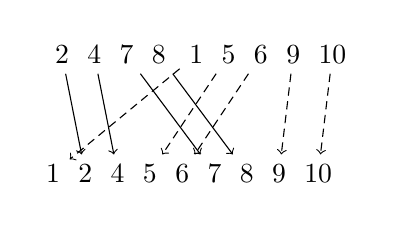
\begin{tikzpicture}
			% Lists
			\matrix[list] (a) at (-1,0) {
				2 & 4 & 7 & 8\\
			};
			\matrix[list] (b) at (1,0) {
				1 & 5 & 6 & 9 & 10\\
			};
			\matrix[list] (c) at (0,-1.5) {
				1 & 2 & 4 & 5 & 6 & 7 & 8 & 9 & 10\\
			};
			
			% Draw arrows from a to c
			\draw[->] (a-1-1) -- (c-1-2);
			\draw[->] (a-1-2) -- (c-1-3);
			\draw[->] (a-1-3) -- (c-1-6);
			\draw[->] (a-1-4) -- (c-1-7);
			
			% Draw arrows from b to c
			\draw[densely dashed, ->] (b-1-1) -- (c-1-1);
			\draw[densely dashed, ->] (b-1-2) -- (c-1-4);
			\draw[densely dashed, ->] (b-1-3) -- (c-1-5);
			\draw[densely dashed, ->] (b-1-4) -- (c-1-8);
			\draw[densely dashed, ->] (b-1-5) -- (c-1-9);
		\end{tikzpicture}
		\caption{Sorted list merging. A typical imperative implementation would invoke a loop over both lists, using appropriate indices for each list. What about recursion?}
		\label{fig:sorted list merging}
	\end{marginfigure}
	
	Having implemented the key operation of sorted list merging and list splitting, the actual implementation of merge sort requires me(a)gre effort\footnote{Cheap wordplay with merge and meagre, in case it went unnoticed\ldots}. So, since we are at it:
	\begin{exercise}\label{ex:merge sort}
		Implement merge sort as a Haskell function \code{mergeSort}. You can (and, maybe, should), utilise \code{merge} from Exercise~\ref{ex:merge} and \code{splitAt'} from Exercise~\ref{ex:split at}. Consider how splitting and then merging will be implemented using recursion.
	\end{exercise}
	%
	%
	%
	\section{Pancake Sorting}
	%
	Do you like pancakes? Well, regardless of your likings, you are requested to sort a heap of pancakes, as the one shown in Figure~\ref{fig:pancakes heap}. More formally, assume you are given a heap of $n$ pancakes, with radiuses from $1$ up to $n$ (pairwise different) placed one on top of the other at any order. Left here, the problem is efficiently (optimally, actually) addressed by merge sort. However, since we are talking about pancakes, we further assume that the only way we are allowed to reorder them is by using a spatula. Thus, we can only flip any top part of the pancake heap.
	
	\begin{marginfigure}
		\centering
		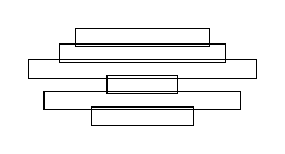
\begin{tikzpicture}
			\foreach [evaluate=\pwidth as \pw using 2*\pwidth+5] \i/\pwidth in {0.0/4, 0.2/10, 0.4/2, 0.6/12, 0.8/8, 1.0/6} {
				\node[draw, rectangle, minimum width={\pw mm}, minimum height=2mm] (p \i) at (0,\i) {};
			}
		\end{tikzpicture}
		\caption{A heap of pancakes, awaiting to be sorted.}
		\label{fig:pancakes heap}
	\end{marginfigure}

	\begin{exercise}\label{ex:pancake sort brainstorming}
		Devise an algorithm that solves the pancake sorting problem described above, i.e., sorts a heap of pancakes by just flipping its top parts (of any length). You can also try to describe it in pseudocode or even implement it in any language you feel more comfortable with, besides Haskell, of course, to verify that your approach actually works.
	\end{exercise}

	\begin{marginfigure}
		\centering
		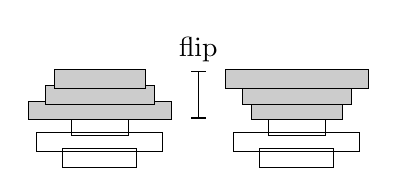
\begin{tikzpicture}
			\foreach [evaluate=\pwidth as \pw using 1.1*\pwidth+5] \i/\pwidth in {0.0/4, 0.2/10, 0.4/2, 0.6/12, 0.8/8, 1.0/6} {
				\ifthenelse{\lengthtest{\i pt < 0.5pt}}{%
					\node[draw, fill=none, rectangle, minimum width={\pw mm}, minimum height=2mm] (p \i) at (0,\i) {};
				}{
					\node[draw, fill=black!20, rectangle, minimum width={\pw mm}, minimum height=2mm] (p \i) at (0,\i) {};
				}
			}
			%
			\foreach [evaluate=\pwidth as \pw using 1.1*\pwidth+5] \i/\pwidth in {0.0/4, 0.2/10, 0.4/2, 0.6/6, 0.8/8, 1.0/12} {
				\ifthenelse{\lengthtest{\i pt < 0.5pt}}{%
					\node[draw, fill=none, rectangle, minimum width={\pw mm}, minimum height=2mm] (p \i) at (2.5,\i) {};
				}{
					\node[draw, fill=black!20, rectangle, minimum width={\pw mm}, minimum height=2mm] (p \i) at (2.5,\i) {};
				}
			}
		
			\draw[|-|] (1.25,0.5) -- (1.25,1.1) node[pos=1, above, text=black] {flip};
		\end{tikzpicture}
		\caption{A valid ``spatula flip'' for pancake sorting.}
		\label{fig:pancakes σορτ}
	\end{marginfigure}

	\begin{exercise}
		Implement the algorithm you developed in Exercise~\ref{ex:pancake sort brainstorming} as a Haskell function using recursion. Before proceeding to the actual implementation, try to figure out the following:
		\begin{itemize}
			\item What should be the base case for this problem?
			\item How can the solution for $n$ be reduced to the solution for some smaller value of $n$, e.g., $n-1$?
		\end{itemize}
		You can hard--code some pancake permutations in order to test your implementation.
	\end{exercise}
	%
	%
	%
	\appendix
	%
	\section{Random Permutations vs Sorting}
	%
	So far, we have generated a random permutation by hard--coding it into our codebase. However, a lot of interesting and efficient algorithms do exist for generating random permutations of lists of integers. Probably the most well known, \href{https://en.wikipedia.org/wiki/Fisher%E2%80%93Yates_shuffle}{Fisher-Yates}, is a common efficient way to implement random shuffling in $O(n)$. However, its implementation requires the active utilisation of static arrays, which are not that straightforward to implement in Haskell. As a substitute, we can think of random shuffling as essentially sorting towards a not necessarily linearly sorted list (in the ordinary sense). Thus, we can utilise any sorting algorithm, in particular merge sort, as developed in Exercise~\ref{ex:merge sort}, to implement an almost equally efficient random shuffling algorithm in Haskell, with the added advantage of guaranteed lack of impurities --- besides randomness, of course.
	
	\begin{exercise}\label{ex:merge shuffle}
		Think of an algorithm that could be utilised in order to shuffle a list by improvising on merge sort. The key here is to ensure equal probability across all possible permutations. \textit{Hint:} Just choosing at random when merging does not suffice. Can you see why?
	\end{exercise}

	\begin{exercise}
		Implement the algorithm you devised in Exercise~\ref{ex:merge shuffle}. To do so, you will need a way to generate random numbers in Haskell, which can be efficiently done using the \code{Random} monad\footnote{A monad is something we are going to study later on this semester. Till then, you can think of them as ``wrappers'' that ensure some certain sort of impurity (e.g., user input / output) stays within certain boundaries, not ``polluting'' the rest of the program.} from the \code{Control} class, i.e., \code{Control.Monad.Random}. To generate random integers in a closed range $[a,b]$, just use \code{getRandomR (a, b)}. You might also want to consider wrapping everything around a custom monad, by declaring the type \code{type R a = Rand StdGen a} or simply using the \code{IO} monad.
	\end{exercise}
	%
	%
	%
\end{document}

